\chapter{Órbitas de fotones, espacio de Rindler e interior de Schwarzschild}

Una masa puntual newtoniana y un agujero negro de Schwarzschild parten de la misma idealización: toda la masa gravitante está concentrada en el centro. Sin embargo, sus centros tienen significados muy distintos. En mecánica newtoniana, una partícula con siquiera un poco de momento angular evita el centro. En un agujero negro, una vez que la partícula ha cruzado el horizonte, no puede evitar la singularidad. Para entender esta diferencia, estudiaremos las órbitas circulares, la esfera de fotones y, por último, un nuevo sistema de coordenadas cerca del horizonte.

\section{Un centro que no se puede evitar}

La materia newtoniana real nunca llega a ser un punto matemático. La presión, la resistencia de los materiales y otras fuerzas se oponen a la compresión. Aunque, pese a ello, usemos una masa puntual como idealización, rara vez una partícula que cae choca con ella. Una trayectoria exactamente radial puede llegar a \(r=0\), pero la menor velocidad transversal aporta momento angular. La barrera centrífuga hace entonces que la partícula dé la vuelta alrededor del centro.

La relatividad general cambia la conclusión. Un cuerpo suficientemente compacto puede formar un agujero negro, y el interior del agujero negro impide la escapatoria newtoniana alrededor del centro. La razón es más profunda que una fuerza más intensa: dentro del horizonte, disminuir \(r\) es una dirección hacia el futuro. Llegaremos a esta afirmación gradualmente, en lugar de darla por supuesta.

\begin{classroomqa}
\audiencequestion{¿La dificultad newtoniana para alcanzar el centro se debe simplemente a que ambos objetos se tratan como puntos?}
\lecturerresponse{La idealización puntual forma parte de la comparación, pero no es toda la diferencia. En mecánica newtoniana, cualquier momento angular distinto de cero permite que la órbita pase alrededor del punto. En el interior relativista, la singularidad está en el futuro de toda trayectoria temporal de caída; el movimiento angular no permite escapar.
\lecturetimestamp{00:04:52--00:05:13}}
\end{classroomqa}

\section{Horizonte y singularidad}

Por ahora, tomaremos como dada la geometría de Schwarzschild:
\begin{equation}
d\tau^{2}
=
\left(1-\frac{2MG}{r}\right)dt^{2}
-
\frac{dr^{2}}{1-\frac{2MG}{r}}
-
r^{2}d\Omega^{2}.
\label{eq:l6-schwarzschild}
\end{equation}
Más adelante veremos las ecuaciones de campo que determinan esta métrica. Nuestra tarea inmediata es aprender qué nos dice.

La métrica de la esfera unidad puede escribirse como
\begin{equation}
d\Omega^{2}
=d\vartheta^{2}+\cos^{2}\vartheta\,d\phi^{2}
\label{eq:l6-angular-metric}
\end{equation}
cuando \(\vartheta\) es la latitud medida desde el plano ecuatorial. Con el ángulo polar más habitual, medido desde el eje, el coseno se convierte en seno. La simetría esférica permite situar cualquier órbita en un plano fijo, de modo que en el cálculo siguiente solo quedará una coordenada angular.

\begin{figure}[htbp]
\centering
\includegraphics[width=0.88\textwidth]{lecture_06_figure_01.png}
\caption{La métrica de Schwarzschild y la representación cilíndrica del espacio-tiempo de la superficie \(r=2MG\). La línea central es \(r=0\); el cilindro rojo es el horizonte en las coordenadas de Schwarzschild.}
\lectureframe{00:09:45}
\end{figure}

Lejos de la fuente, \(2MG/r\) es pequeño y la ec.~\eqref{eq:l6-schwarzschild} se aproxima a la métrica de Minkowski en coordenadas esféricas. Destacan dos radios:
\begin{equation}
r=2MG,
\qquad
r=0.
\end{equation}
No hay que confundirlos. En \(r=2MG\), el coeficiente de \(dt^{2}\) se anula y el de \(dr^{2}\) diverge. El sistema de coordenadas de Schwarzschild se ha vuelto singular. Allí la curvatura sigue siendo finita. En cambio, en \(r=0\) divergen los invariantes de curvatura. El campo de marea estira radialmente un cuerpo extenso y lo comprime transversalmente sin límite. Se trata de una singularidad física, no de un defecto de las coordenadas.

\subsection{Dos maneras de medir el tiempo de una caída}

Para un reloj estacionario fuera del horizonte,
\begin{equation}
d\tau
=
\sqrt{1-\frac{2MG}{r}}\,dt.
\label{eq:l6-static-clock}
\end{equation}
A grandes \(r\), \(d\tau\simeq dt\). Cerca del horizonte, el tiempo propio de un reloj mantenido en un \(r\) fijo transcurre muy lentamente con respecto al tiempo de Schwarzschild medido lejos de allí.

Con estas mismas coordenadas, la caída radial tarda un valor infinito de \(t\) en llegar a \(r=2MG\). El tiempo propio transcurrido para quien cae es finito. No hay contradicción entre ambas afirmaciones. El reloj que lleva quien cae mide el tiempo propio a lo largo de su línea de universo. Puede ser un reloj mecánico, un reloj de luz hecho con espejos en los extremos de una regla de un metro, un latido o la sucesión de procesos físicos en un cerebro. Ninguno de ellos mide el tiempo de coordenadas distante \(t\). La diferencia entre ambos relojes se hará visible en el diagrama cerca del horizonte.

\section{Movimiento circular a partir de la acción de tiempo propio}

Antes de volver a la caída, resolvamos otro problema: ¿en qué condiciones puede una partícula masiva o un fotón dar vueltas alrededor del agujero negro? El cálculo comienza con el mismo principio de acción que se usa para cualquier partícula relativista en movimiento libre,
\begin{equation}
S=-m\int d\tau.
\label{eq:l6-particle-action}
\end{equation}
La Tierra desvía la luz, pero su campo está muy lejos de ser lo bastante intenso como para curvar un rayo de luz hasta cerrarlo en una órbita. El radio de Schwarzschild de la Tierra es del orden de un centímetro. Habría que comprimir toda la Tierra hasta aproximadamente esa escala, más o menos el tamaño de una nuez pequeña, para que la cuestión del campo intenso fuese pertinente.

Fijemos \(c=1\), restrinjamos el movimiento al plano ecuatorial y definamos
\begin{equation}
F(r)=1-\frac{2MG}{r},
\qquad
G(r)=\frac{1}{F(r)}.
\label{eq:l6-fg}
\end{equation}
Al tomar el tiempo de coordenadas \(t\) como parámetro, se obtiene
\begin{equation}
d\tau
=dt\sqrt{F-G\dot r^{\,2}-r^{2}\dot\theta^{\,2}},
\end{equation}
y, por tanto,
\begin{equation}
\mathcal L
=
-m\sqrt{F-G\dot r^{\,2}-r^{2}\dot\theta^{\,2}}.
\label{eq:l6-lagrangian}
\end{equation}
El factor \(m\) da a la acción sus dimensiones habituales de energía por tiempo.

\begin{figure}[htbp]
\centering
\includegraphics[width=0.76\textwidth]{lecture_06_figure_02.png}
\caption{El lagrangiano de la partícula, con su raíz cuadrada, se construye en la pizarra. La expresión completa aparece en la ec.~\eqref{eq:l6-lagrangian}.}
\lectureframe{00:31:53}
\end{figure}

Para cualquier coordenada generalizada \(q\),
\begin{equation}
p_q=\frac{\partial\mathcal L}{\partial\dot q}.
\end{equation}
Conviene reservar \(\mathcal L\) para el lagrangiano y \(L\) para el momento angular. Con
\begin{equation}
\Delta=F-G\dot r^{\,2}-r^{2}\dot\theta^{\,2},
\end{equation}
los dos momentos son
\begin{align}
L=p_\theta
&=\frac{mr^{2}\dot\theta}{\sqrt{\Delta}},
\label{eq:l6-angular-momentum}\\
p_r
&=\frac{mG\dot r}{\sqrt{\Delta}}.
\label{eq:l6-radial-momentum}
\end{align}
El momento radial no se conserva porque la coordenada radial aparece en el lagrangiano. El ángulo \(\theta\) no aparece, así que \(L\) se conserva.

Además, \(t\) no aparece explícitamente en \(\mathcal L\). Por tanto, el hamiltoniano se conserva:
\begin{align}
E=H
&=p_r\dot r+L\dot\theta-\mathcal L \\
&=\frac{mG\dot r^{\,2}}{\sqrt{\Delta}}
  +\frac{mr^{2}\dot\theta^{\,2}}{\sqrt{\Delta}}
  +m\sqrt{\Delta} \\
&=\frac{mF}{\sqrt{\Delta}}.
\label{eq:l6-energy-general}
\end{align}
Este es un ritmo característico de la mecánica. Un principio da la acción; un cálculo da los momentos; y luego la simetría transforma el cálculo en los principios de conservación de la energía y del momento angular. Podríamos resolver de inmediato todas las ecuaciones de Euler--Lagrange, pero las constantes que proporciona la simetría rotacional y la de traslación temporal eliminan buena parte de ese trabajo.

\subsection{La energía de la órbita circular}

Para una órbita circular,
\begin{equation}
\dot r=0.
\end{equation}
Introduzcamos el momento angular por unidad de masa,
\begin{equation}
\lambda=\frac{L}{m}.
\end{equation}
Las ecuaciones~\eqref{eq:l6-angular-momentum} y \eqref{eq:l6-energy-general} se convierten en
\begin{align}
\lambda
&=\frac{r^{2}\dot\theta}
{\sqrt{F-r^{2}\dot\theta^{\,2}}},
\label{eq:l6-lambda-circular}\\
E
&=\frac{mF}{\sqrt{F-r^{2}\dot\theta^{\,2}}}.
\label{eq:l6-energy-circular-first}
\end{align}

\begin{figure}[htbp]
\centering
\includegraphics[width=0.82\textwidth]{lecture_06_figure_04.png}
\caption{El momento angular reducido y la energía del movimiento circular de Schwarzschild. Primero se usa la ecuación del momento angular para eliminar \(\dot\theta\) de la energía.}
\lectureframe{00:39:14}
\end{figure}

Elevando al cuadrado la ec.~\eqref{eq:l6-lambda-circular} y despejando la velocidad angular, se obtiene
\begin{equation}
\dot\theta^{\,2}
=
\frac{\lambda^{2}F}
{r^{2}\left(r^{2}+\lambda^{2}\right)}.
\label{eq:l6-angular-speed}
\end{equation}
Al sustituir en la ec.~\eqref{eq:l6-energy-circular-first}, queda una energía que depende solo del radio propuesto y del momento angular fijo:
\begin{equation}
E(r,\lambda)
=m\sqrt{F(r)}\,\frac{\sqrt{r^{2}+\lambda^{2}}}{r}.
\label{eq:l6-circular-energy}
\end{equation}

La clase se detiene para comparar con el caso newtoniano. En una órbita circular ordinaria, la frecuencia angular y la velocidad tangencial disminuyen al aumentar el radio, pero el momento angular incluye un factor de radio. Por tanto, no se debe inferir el comportamiento de \(L\) a partir únicamente de la velocidad angular. La fórmula relativista deja explícitos esos factores.

\section{La órbita circular de la luz}

Un fotón tiene energía y momento aunque su masa en reposo sea nula. Por tanto, el límite sin masa de la ec.~\eqref{eq:l6-circular-energy} debe tomarse con cuidado. Si \(m\) tendiera a cero manteniendo fijo \(\lambda\), también se anularía \(L=m\lambda\). En su lugar, tomemos
\begin{equation}
m\longrightarrow0,
\qquad
\lambda\longrightarrow\infty,
\qquad
L=m\lambda\ \text{fixed}.
\label{eq:l6-massless-limit}
\end{equation}
En ese caso, domina el término \(\lambda^{2}\) y la energía del fotón pasa a ser
\begin{equation}
E_\gamma(r;L)
=L\,\frac{\sqrt{1-\frac{2MG}{r}}}{r}.
\label{eq:l6-photon-energy}
\end{equation}
El factor \(L\) multiplica toda la función radial. Afecta la escala de energía, pero no el radio de una órbita circular.

\begin{figure}[htbp]
\centering
\includegraphics[width=0.88\textwidth]{lecture_06_figure_05.png}
\caption{El factor radial de la energía del fotón. Se anula en el horizonte, tiende a cero a grandes radios y tiene un máximo entre ambos.}
\lectureframe{00:50:50}
\end{figure}

A \(L\) fijo, el equilibrio radial exige un punto estacionario:
\begin{equation}
\frac{d}{dr}
\left[
\frac{\sqrt{1-\frac{2MG}{r}}}{r}
\right]=0.
\end{equation}
Al derivar,
\begin{equation}
-\frac{\sqrt{1-\frac{2MG}{r}}}{r^{2}}
+
\frac{MG}
{r^{3}\sqrt{1-\frac{2MG}{r}}}
=0,
\end{equation}
y, por tanto,
\begin{equation}
r=3MG.
\label{eq:l6-photon-sphere}
\end{equation}
Este radio es una vez y media el radio de Schwarzschild. Suele llamarse esfera de fotones.

El punto estacionario es un máximo, así que la órbita circular del fotón es inestable. Un fotón situado exactamente en \(3MG\) permanece allí. Un desplazamiento radial arbitrariamente pequeño acaba alejándolo del máximo. Justo fuera de la esfera de fotones, un rayo puede recorrer un ángulo muy grande, quizá dar muchas vueltas alrededor del agujero, antes de escapar. Justo dentro, un rayo casi tangencial puede dar varias vueltas y luego caer a través del horizonte.

\begin{figure}[htbp]
\centering
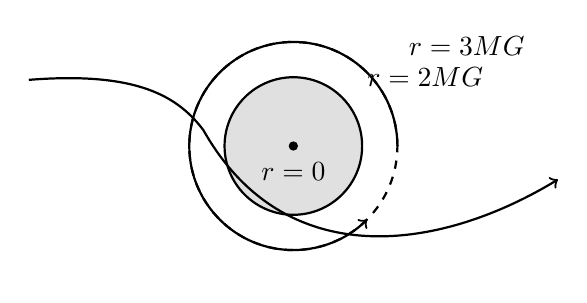
\begin{tikzpicture}[scale=1.12]
\fill[black!12] (0,0) circle (0.78);
\draw[thick] (0,0) circle (0.78);
\draw[dashed,thick] (0,0) circle (1.18);
\fill (0,0) circle (1.5pt);
\draw[->,thick] (1.18,0) arc (0:315:1.18);
\draw[->,thick] (-3.0,0.75)
  .. controls (-1.75,0.85) and (-1.30,0.55) .. (-1.02,0.18)
  .. controls (-0.10,-1.45) and (1.65,-1.20) .. (3.0,-0.38);
\node[right] at (0.73,0.78) {\(r=2MG\)};
\node[right] at (1.20,1.13) {\(r=3MG\)};
\node[below] at (0,-0.08) {\(r=0\)};
\end{tikzpicture}
\caption{El horizonte, la esfera de fotones y un rayo fuertemente desviado. Los rayos que pasan arbitrariamente cerca de la órbita circular inestable pueden acumular una desviación arbitrariamente grande antes de escapar o caer hacia dentro.}
\end{figure}

\begin{classroomqa}
\audiencequestion{¿Por qué se mantiene fijo el momento angular y cómo se relaciona con la frecuencia y la trayectoria de entrada de un fotón?}
\lecturerresponse{Todo rayo lleva un momento angular conservado con respecto al agujero negro. Su frecuencia determina el módulo de su momento lineal, mientras que su distancia de paso respecto al centro contribuye a determinar \(L\). Fuera de una órbita circular, el radio y el momento angular pueden elegirse independientemente. Exigir una órbita circular del fotón vincula el movimiento al radio único \(3MG\), y la factorización de la ec.~\eqref{eq:l6-photon-energy} muestra que ese radio es independiente del módulo de \(L\).
\lecturetimestamp{00:54:43--00:57:02}}
\end{classroomqa}

\begin{classroomqa}
\audiencequestion{¿Por qué el máximo de la energía determina una órbita?}
\lecturerresponse{Una vez eliminado el movimiento angular a \(L\) fijo, la función restante desempeña el papel de una energía radial efectiva. Un punto estacionario proporciona equilibrio radial. Un mínimo sería estable; este punto es un máximo y, por tanto, da una órbita circular inestable. No hay contradicción en llamarlo equilibrio e inestable al mismo tiempo.
\lecturetimestamp{00:57:51--00:58:54}}
\end{classroomqa}

Una partícula masiva puede tener órbitas circulares temporales fuera de \(3MG\), aunque las más cercanas a la esfera de fotones son inestables. Una partícula sin masa solo tiene la órbita circular en \(3MG\). Dentro de la esfera de fotones, un fotón que se mueve tangencialmente cae hacia dentro; un objeto que se mueve más despacio no tiene mejores posibilidades de mantener una órbita así. Esta afirmación se refiere al movimiento angular. Fuera del horizonte, un rayo con dirección suficientemente hacia fuera aún puede escapar aunque su radio inicial sea menor que \(3MG\).

\section{Qué le hace un agujero negro a una imagen}

La esfera de fotones explica por qué un agujero negro no es simplemente un disco oscuro superpuesto a un cielo que, por lo demás, no cambia. La luz de un objeto de fondo puede llegar a un observador por varias trayectorias. Un rayo puede pasar por un lado del agujero, otro por el lado opuesto y otros pueden dar una o más vueltas a su alrededor. El resultado puede incluir imágenes desplazadas, duplicadas, anillos y una secuencia infinita de imágenes cada vez más pequeñas y tenues, asociadas a vueltas adicionales. La imagen exacta es complicada, pero su origen ya está contenido en la órbita inestable.

Cuando la fuente, la lente y el observador están suficientemente alineados, la imagen puede formar un anillo de Einstein. En la naturaleza se observan anillos de lente gravitacional. Para obtener la imagen completa del agujero negro hay que integrar las geodésicas nulas para muchas direcciones iniciales, un cálculo muy apropiado para una computadora.

\begin{classroomqa}
\audiencequestion{¿Este límite óptico se refiere a la esfera de fotones o al horizonte?}
\lecturerresponse{Cumplen funciones distintas. El horizonte en \(2MG\) es el límite causal: ninguna señal dirigida hacia el futuro escapa desde su interior. La esfera de fotones en \(3MG\) controla el movimiento tangencial y las lentes gravitacionales intensas. Entre ambos radios, un rayo radial hacia fuera puede escapar, mientras que un rayo tangencial cae hacia dentro. Las direcciones intermedias pueden dar vueltas antes de escapar o ser capturadas.
\lecturetimestamp{01:02:47--01:03:40}}
\end{classroomqa}

\begin{classroomqa}
\audiencequestion{¿Se puede calcular una trayectoria de luz general, en lugar de limitarse a esbozarla?}
\lecturerresponse{Sí. Se introduce la condición nula en las ecuaciones geodésicas o de Euler--Lagrange y se integra con los datos iniciales elegidos. Las ecuaciones no son conceptualmente nuevas, pero el trazado de rayos resulta algebraicamente engorroso, por lo que el cálculo numérico es el método práctico para obtener una imagen.
\lecturetimestamp{01:03:48--01:04:27}}
\end{classroomqa}

\begin{classroomqa}
\audiencequestion{¿Habría sido más difícil calcular la órbita circular aplicando directamente las ecuaciones de Euler--Lagrange?}
\lecturerresponse{Se obtendría el mismo resultado. En ambos métodos, la acción es el punto de partida adecuado, pero las coordenadas cíclicas ponen de manifiesto la energía y el momento angular conservados. Usar primero esas constantes es la vía más breve para obtener la condición de órbita circular.
\lecturetimestamp{01:04:33--01:05:49}}
\end{classroomqa}

\section{La métrica cerca del horizonte es el espacio de Rindler}

Volvamos ahora al horizonte. Allí los coeficientes de Schwarzschild parecen divergir o anularse, y al cruzar el horizonte intercambian sus signos. Sin embargo, un observador en caída no encuentra una curvatura local divergente en esa superficie. El principio de equivalencia nos indica cómo pueden ser ciertas ambas afirmaciones.

Empecemos con el espacio-tiempo de Minkowski bidimensional:
\begin{equation}
d\tau^{2}=dT^{2}-dX^{2}.
\end{equation}
En la cuña derecha de Rindler, definamos
\begin{equation}
X=\rho\cosh\omega,
\qquad
T=\rho\sinh\omega.
\label{eq:l6-rindler-map}
\end{equation}
Las curvas de \(\rho\) constante cumplen
\begin{equation}
X^{2}-T^{2}=\rho^{2},
\end{equation}
por lo que son hipérbolas: las líneas de universo de observadores con aceleración uniforme. Al sustituir la ec.~\eqref{eq:l6-rindler-map} en la métrica plana, se obtiene
\begin{equation}
d\tau^{2}
=\rho^{2}d\omega^{2}-d\rho^{2}.
\label{eq:l6-rindler-metric}
\end{equation}
Ahora fijemos
\begin{equation}
\rho^{2}=4\xi,
\qquad
\omega=\frac{t}{2}.
\label{eq:l6-rindler-rescale}
\end{equation}
Como \(d\rho^{2}=d\xi^{2}/\xi\), la ec.~\eqref{eq:l6-rindler-metric} se convierte en
\begin{equation}
d\tau^{2}
=\xi\,dt^{2}-\frac{d\xi^{2}}{\xi}.
\label{eq:l6-xi-metric}
\end{equation}

\begin{classroomqa}
\audiencequestion{¿Adónde han ido las coordenadas angulares o transversales?}
\lecturerresponse{Solo las hemos omitido. Estamos examinando el plano local \(t\)-\(r\) que contiene el comportamiento al cruzar el horizonte. Las dos direcciones transversales siguen siendo regulares y se pueden reintroducir; no cambian la singularidad de coordenadas que estamos analizando.
\lecturetimestamp{01:16:27--01:16:47}}
\end{classroomqa}

Para comparar con Schwarzschild, elijamos unidades en las que \(2MG=1\). La parte radial de la ec.~\eqref{eq:l6-schwarzschild} es
\begin{equation}
d\tau^{2}
=
\frac{r-1}{r}\,dt^{2}
-
\frac{r}{r-1}\,dr^{2}.
\end{equation}
Muy cerca de \(r=1\), hay que conservar el pequeño numerador \(r-1\), mientras que los factores \(r\), inocuos en los demás casos, pueden sustituirse por uno. Así,
\begin{equation}
d\tau^{2}
\simeq
(r-1)\,dt^{2}
-
\frac{dr^{2}}{r-1}.
\end{equation}
Con
\begin{equation}
\xi=r-1,
\end{equation}
esta es exactamente la ec.~\eqref{eq:l6-xi-metric}. La geometría de Schwarzschild cerca del horizonte es, localmente, la descripción de Minkowski plano en coordenadas de Rindler.

\begin{classroomqa}
\audiencequestion{¿Cómo pueden ser coordenadas aceleradas si el espacio-tiempo subyacente es plano?}
\lecturerresponse{La aceleración corresponde al observador, no necesariamente a la curvatura. Una línea de universo con \(\rho\) fijo tiene aceleración uniforme en el espacio-tiempo de Minkowski. Del mismo modo, un observador mantenido a radio fijo cerca de un agujero negro debe estar sostenido contra la caída libre. El principio de equivalencia hace que las descripciones locales concuerden, aunque el espacio-tiempo de Schwarzschild completo sea curvo.
\lecturetimestamp{01:22:19--01:24:06}}
\end{classroomqa}

\section{Cruzar el horizonte de Rindler}

Las fórmulas de la cuña derecha solo cubren \(\xi>0\):
\begin{equation}
X=2\sqrt{\xi}\cosh\frac{t}{2},
\qquad
T=2\sqrt{\xi}\sinh\frac{t}{2}.
\label{eq:l6-rindler-outside}
\end{equation}
La superficie \(\xi=0\) es la línea nula \(X=T\). Para continuar hacia la cuña futura, definamos
\begin{equation}
\zeta=-\xi>0
\end{equation}
e intercambiemos los papeles hiperbólicos:
\begin{equation}
T=2\sqrt{\zeta}\cosh\frac{t}{2},
\qquad
X=2\sqrt{\zeta}\sinh\frac{t}{2}.
\label{eq:l6-rindler-inside}
\end{equation}
La métrica sigue siendo
\begin{equation}
d\tau^{2}
=\xi\,dt^{2}-\frac{d\xi^{2}}{\xi},
\end{equation}
pero cuando \(\xi<0\), el coeficiente de \(dt^{2}\) es negativo y el de \(d\xi^{2}\) es positivo. La coordenada \(\xi\), y por tanto la dirección radial de Schwarzschild, se ha vuelto temporal; \(t\) se ha vuelto espacial.

\begin{figure}[htbp]
\centering
\includegraphics[width=0.88\textwidth]{lecture_06_figure_06.png}
\caption{Las cuñas de Rindler, sus fronteras nulas y la continuación de \(\xi>0\) a \(\xi<0\). En la pizarra también se anotan \(\rho^{2}=4\xi\) y \(\omega=t/2\).}
\lectureframe{01:29:40}
\end{figure}

\begin{classroomqa}
\audiencequestion{¿Algunas curvas de este dibujo de coordenadas se mueven más rápido que la luz?}
\lecturerresponse{Una línea de la cuadrícula de coordenadas no tiene por qué ser la línea de universo de un objeto material. Su pendiente en coordenadas puede parecer superlumínica sin violar la causalidad. Los rayos de luz físicos siguen siendo nulos, y las partículas físicas permanecen dentro de sus conos de luz locales.
\lecturetimestamp{01:28:44--01:29:08}}
\end{classroomqa}

Al continuar hacia el interior de Schwarzschild, finalmente llegamos a \(r=0\). Esa frontera es espacial. Por ello, es mejor describirla como un tiempo que como un lugar: toda trayectoria temporal o nula dirigida hacia el futuro en el interior del agujero negro la alcanza. Se puede rodear un lugar. No se puede rodear el propio futuro.

\begin{classroomqa}
\audiencequestion{¿Podría el diagrama simplemente continuar a través de \(r=0\) hasta un \(r\) negativo, y sigue siendo \(r=0\) el centro?}
\lecturerresponse{El dibujo de coordenadas puede tentar a prolongar una línea, pero la solución clásica de Schwarzschild termina en la singularidad de curvatura. \(r=0\) aún puede llamarse el centro, pero es un centro muy peculiar: en el interior es una frontera futura espacial. No hay un paso regular a través de ella hacia una región de radio negativo.
\lecturetimestamp{01:32:16--01:34:06}}
\end{classroomqa}

\begin{classroomqa}
\audiencequestion{¿Son nulos los ejes diagonales del diagrama de Rindler, y puede quien cae entrar en un valor finito del tiempo acelerado?}
\lecturerresponse{Sí, las fronteras de la cuña son líneas nulas. Una línea de universo en caída libre cruza una de ellas en un suceso ordinario y en un tiempo propio finito. La coordenada acelerada \(t\), o equivalentemente \(\omega\), crece sin límite en la descripción exterior con \(\rho\) constante; lo que se vuelve infinito es esa asignación de coordenadas, no el suceso del cruce.
\lecturetimestamp{01:34:26--01:35:03}}
\end{classroomqa}

\section{Alicia en el exterior y Bob en caída}

Dejemos a Alicia en el exterior, a radio fijo y sostenida contra la gravedad, y hagamos que Bob caiga libremente. Cerca del horizonte, Alicia sigue una hipérbola parecida a la de Rindler. Sus secciones de \(t\) constante se amontonan cada vez más cerca de la frontera nula. Todo suceso de la línea de universo de Bob que Alicia etiqueta con un \(t\) finito queda fuera del horizonte, así que ella nunca asigna un tiempo de Schwarzschild finito a su cruce.

Bob lleva un reloj de tiempo propio. Su trayectoria cruza la línea nula durante un intervalo finito de ese reloj. Al cruzar no ocurre nada localmente divergente. El horizonte es decisivo a escala global, pero localmente es ordinario.

\begin{figure}[htbp]
\centering
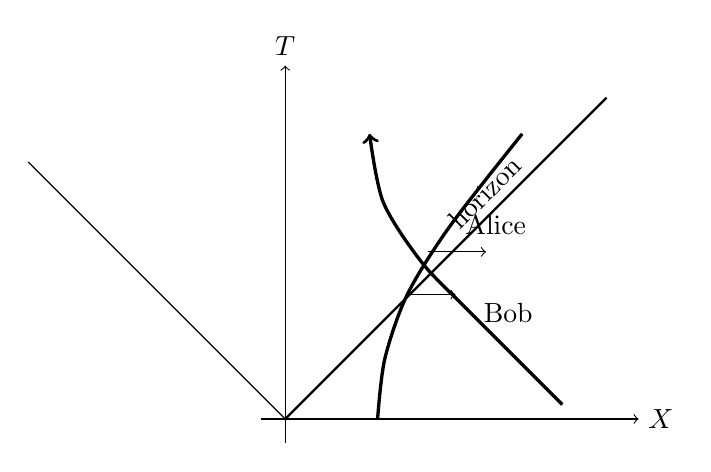
\begin{tikzpicture}[scale=1.02]
\draw[->] (-0.3,0) -- (4.4,0) node[right] {\(X\)};
\draw[->] (0,-0.3) -- (0,4.4) node[above] {\(T\)};
\draw[thick] (0,0) -- (4.0,4.0);
\draw[thin] (0,0) -- (-3.2,3.2);
\node[rotate=45,above] at (2.65,2.65) {horizon};
\draw[very thick]
  plot[smooth] coordinates {(1.15,0.0) (1.24,0.75) (1.52,1.55)
  (2.05,2.40) (2.95,3.55)};
\node[right] at (2.12,2.42) {Alice};
\draw[very thick,->]
  plot[smooth] coordinates {(3.45,0.18) (2.85,0.78) (2.25,1.38)
  (1.70,1.95) (1.22,2.70) (1.05,3.55)};
\node[right] at (2.35,1.32) {Bob};
\draw[->] (1.52,1.55) -- (2.12,1.55);
\draw[->] (1.78,2.08) -- (2.50,2.08);
\end{tikzpicture}
\caption{La línea de universo acelerada de Alicia en el exterior y la línea de universo de Bob en caída libre. Las secciones de coordenadas de Alicia se acercan al horizonte; Bob lo cruza en un tiempo propio finito.}
\end{figure}

\begin{classroomqa}
\audiencequestion{¿Qué ve Bob cuando mira hacia atrás, hacia Alicia, y qué ocurre con su reloj después del cruce?}
\lecturerresponse{Bob ve que Alicia se aleja con la aceleración necesaria para mantenerse en el exterior, pero no ve ningún suceso singular al cruzar. Alicia puede estar sostenida a radio fijo; una órbita es otra configuración posible. El reloj de Bob sigue midiendo normalmente su tiempo propio \(\tau\). En el interior, decir que la coordenada radial es temporal describe la geometría causal; no convierte literalmente su reloj de pulsera en una regla. Su línea de universo termina finalmente en \(r=0\).
\lecturetimestamp{01:39:51--01:44:45}}
\end{classroomqa}

Ahora reconocemos que la línea nula es el horizonte mismo, no simplemente un punto en el que un coeficiente de las coordenadas se comporta mal. Fuera de él, una familia de rayos de luz radiales se mueve hacia fuera. Dentro de él, ambas direcciones futuras del cono de luz llevan hacia valores menores de \(r\). Toda trayectoria futura de un cuerpo masivo debe permanecer entre esas dos direcciones nulas y, por tanto, llega a la singularidad.

\section{Señales, corrimiento al rojo y formación de un horizonte}

Supongamos que la materia en colapso emite una secuencia regular de pulsos de luz. Un observador distante recibe los pulsos posteriores a intervalos cada vez mayores. Sus frecuencias se desplazan desde el óptico hacia el infrarrojo, las microondas, las ondas de radio y longitudes de onda aún mayores. En un cálculo clásico idealizado, el observador exterior puede seguir asociando señales cada vez más tardías con materia que se aproxima al horizonte, pero en la práctica la fuente pronto se vuelve demasiado roja y tenue para detectarla.

\begin{classroomqa}
\audiencequestion{Durante el colapso, ¿ve un observador exterior que toda la materia simplemente se congela en el horizonte?}
\lecturerresponse{En el tiempo de Schwarzschild, la superficie de la materia en colapso se aproxima asintóticamente al horizonte y parece congelarse cada vez más. Lo que realmente se observa está codificado en señales de luz, que llegan con retrasos cada vez mayores, más corridas al rojo y más tenues. Esta descripción en coordenadas no afirma que la materia en caída experimente un tiempo propio infinito.
\lecturetimestamp{01:47:06--01:48:11}}
\end{classroomqa}

\begin{classroomqa}
\audiencequestion{¿Podría un observador que espera lo suficiente recuperar toda la historia de la caída?}
\lecturerresponse{Solo mediante señales que se hayan emitido y consigan llegar al observador. Los pulsos sucesivos están cada vez más separados y más corridos al rojo. Un observador ideal con sensibilidad ilimitada podría seguir la señal clásica hasta longitudes de onda cada vez mayores; un observador práctico ve cómo el objeto se desvanece.
\lecturetimestamp{01:48:13--01:52:00}}
\end{classroomqa}

\begin{classroomqa}
\audiencequestion{¿Qué significa exactamente decir que la singularidad es un tiempo y no un lugar?}
\lecturerresponse{La superficie \(r=0\) es espacial. Una vez dentro del horizonte, toda curva temporal o nula dirigida hacia el futuro termina allí. Se puede evitar una ubicación espacial eligiendo otra ruta; no se puede evitar una frontera futura mientras se sigue una línea de universo dirigida hacia el futuro.
\lecturetimestamp{01:52:02--01:53:10}}
\end{classroomqa}

Entonces, ¿cómo puede formarse un agujero negro o aumentar su masa si el observador exterior nunca ve cruzar la materia? Consideremos una cáscara esférica en colapso. El horizonte global no espera como una superficie material preexistente en un radio fijo. Comienza en el centro y crece hacia fuera hasta encontrarse con la cáscara mientras se forma la región del agujero negro. La descripción externa de Schwarzschild sigue mostrando que la cáscara se aproxima asintóticamente al horizonte final. El tema de la siguiente lección será la imagen completa del espacio-tiempo, incluido el modo de localizar globalmente el horizonte.

\begin{figure}[htbp]
\centering
\includegraphics[width=0.90\textwidth]{lecture_06_figure_07.png}
\caption{Una cáscara en colapso y el horizonte, que crece hacia fuera desde el centro hasta encontrarse con ella. El dibujo anticipa la geometría global del colapso que se desarrollará en la siguiente lección.}
\lectureframe{01:57:25}
\end{figure}

\begin{classroomqa}
\audiencequestion{Si nada cruza el horizonte en el tiempo de coordenadas externo, ¿cómo puede formarse o crecer un agujero negro?}
\lecturerresponse{La premisa mezcla una afirmación sobre coordenadas con una afirmación global. La materia en colapso llega a la región pertinente en un tiempo propio finito, mientras que el horizonte de sucesos está determinado por la estructura causal de todo el espacio-tiempo. En el modelo de la cáscara, comienza en el centro y crece hacia fuera hasta encontrarse con ella. La visión retrasada y corrida al rojo del observador exterior sigue siendo compatible con ese horizonte global.
\lecturetimestamp{01:53:11--01:57:34}}
\end{classroomqa}

\section{Direcciones de escape entre las dos esferas}

El horizonte y la esfera de fotones dividen el problema de los rayos en casos distintos. A un radio
\begin{equation}
2MG<r<3MG,
\end{equation}
un rayo de luz radial hacia fuera puede escapar al infinito. Un rayo tangencial no puede: cae hacia dentro. Entre esas direcciones hay un cono de escape. Cuanto más cerca del horizonte, más se estrecha ese cono alrededor de la dirección radial hacia fuera. Una vez cruzado el horizonte, se cierra por completo.

\begin{classroomqa}
\audiencequestion{¿Puede una fuente de luz entre el horizonte y la esfera de fotones enviar alguna señal hacia fuera?}
\lecturerresponse{Sí. Un rayo nulo suficientemente radial y dirigido hacia fuera escapa siempre que su suceso de emisión esté fuera de \(2MG\). La afirmación de que el movimiento angular dentro de \(3MG\) cae hacia dentro no impide el escape radial. El resultado depende de la dirección de emisión, y el cono de direcciones permitidas hacia fuera se estrecha al acercarse la fuente al horizonte.
\lecturetimestamp{01:57:34--01:59:48}}
\end{classroomqa}

\begin{classroomqa}
\audiencequestion{¿Puede un rayo que llega desde el exterior cruzar al interior de la esfera de fotones, darse la vuelta y volver a salir?}
\lecturerresponse{No a lo largo de una geodésica nula del tipo que estamos considerando. En un punto de retorno la velocidad radial sería cero, por lo que el rayo sería momentáneamente tangencial a un radio menor que \(3MG\); allí, la trayectoria angular cae hacia dentro en vez de volver hacia fuera. Sin embargo, una fuente situada entre las dos esferas puede emitir un rayo suficientemente radial hacia fuera antes de cruzar el horizonte.
\lecturetimestamp{01:59:49--02:01:27}}
\end{classroomqa}

La última pregunta queda deliberadamente menos resuelta. Imaginemos que Alice y Bob se mantienen ambos a la misma distancia radial, fuera del horizonte. Los observadores cercanos pueden intercambiar señales sin dificultad. Si están muy separados alrededor de la esfera, el trayecto nulo directo y el límite de su alcance angular requieren un cálculo geodésico explícito. En clase se propone una ruta indirecta: enviar el mensaje casi radialmente hacia fuera hasta un repetidor situado a una distancia radial más segura, llevarlo por allí y enviarlo de vuelta hacia dentro. Otra variante permite que un objeto lanzado hacia fuera, o una señal, dé la vuelta y regrese. Estas rutas muestran por qué la imposibilidad de una órbita circular tangencial no prohíbe por sí sola toda comunicación entre observadores exteriores.

\begin{classroomqa}
\audiencequestion{¿Pueden comunicarse alrededor del agujero negro dos observadores suspendidos a la misma distancia radial, cerca del horizonte?}
\lecturerresponse{Localmente, sí. Para observadores muy separados o diametralmente opuestos, el límite del trayecto directo no se calculó en la clase y no debe presentarse como un teorema. Primero, la discusión deja abierta esa cuestión de las geodésicas angulares; luego, observa que una señal indirecta puede viajar casi radialmente hacia fuera, ser retransmitida a una distancia radial mayor y regresar. Al acercarse al horizonte, el alcance angular útil para la comunicación directa se estrecha cada vez más, pero fuera del horizonte sigue habiendo una ruta hacia fuera.
\lecturetimestamp{02:01:29--02:04:17}}
\end{classroomqa}

El siguiente paso consiste en sustituir estos esquemas cerca del horizonte por la geometría global de un cuerpo en colapso y determinar con precisión cómo crece un horizonte de sucesos.